{}\documentclass[letterpaper,
compress,
xcolor=x11names,
%draft,
]{beamer}
% Package imports
\usepackage{mathtools} % imports `amsmath'
\DeclareMathOperator{\sech}{sech}
\usepackage{amssymb}
\usepackage{fixltx2e}
\usepackage{lmodern}
\usepackage{movie15}
%\usepackage{media9}
\usepackage{microtype}
\usepackage{animate}
\usepackage{subcaption}
\captionsetup{compatibility=false}

% I just did this
\usepackage[english]{babel}
\usepackage[utf8]{inputenc}
\usepackage{amsmath}
\usepackage{graphicx}
\usepackage[colorinlistoftodos]{todonotes}
\usepackage{tikz}
\usetikzlibrary{tikzmark}
\usepackage{array}
\usepackage{layout}
\usepackage{multicol}
\usepackage{multirow}
\usepackage{booktabs}
%I just did this

% `beamer' configuration
\usefonttheme{professionalfonts}
\useoutertheme[subsection=false,]{miniframes}
\setbeamercolor*{alerted text}{fg=red}
\setbeamercolor*{example text}{fg=black}
\definecolor{CSU_green}{RGB}{30, 70, 43}
\definecolor{CSU_gold}{RGB}{200, 195, 114}
\setbeamercolor*{lower separation line head}{bg=CSU_gold}
\setbeamercolor*{section in head/foot}{fg=white,bg=CSU_green}
\setbeamercolor*{subsection in head/foot}{bg=white}
\setbeamercolor*{upper separation line head}{bg=CSU_gold}
\setbeamercolor*{page number in head/foot}{fg=CSU_green}
\setbeamercolor*{normal text}{fg=black,bg=white}
\setbeamercolor*{palette tertiary}{fg=black,bg=black!10}
\setbeamercolor*{palette quaternary}{fg=black,bg=black!10}
\setbeamercolor*{structure}{fg=black}
\setbeamerfont{frametitle}{shape=\scshape}
\setbeamerfont{institute}{shape=\scshape}
\setbeamerfont{section in head/foot}{shape=\scshape}
\setbeamerfont{subsection in head/foot}{shape=\scshape}
\setbeamertemplate{bibliography item}{}
\setbeamertemplate{itemize items}[ball]
\setbeamertemplate{navigation symbols}{}
\setbeamertemplate{footline}[frame number]
\usetikzlibrary{calc,arrows}
\graphicspath{{graphics/}{graphics/movies/}{graphics/images/}}
\usepackage{remreset}                  % hack to display beamer navigation
\makeatletter                          % circles even if not declaring
\@removefromreset{subsection}{section} % subsections
\makeatother                           % see: http://tex.stackexchange.com/a/2078
\setcounter{subsection}{1}             % see: https://bitbucket.org/rivanvx/beamer/issue/218

% `biblatex' configuration
\usepackage[backend=biber,
style=authortitle-comp,
]{biblatex}
\addbibresource{presentation.bib}

% `enumitem' configuration
\usepackage{enumitem}
\setlist[itemize,1]{label=\usebeamertemplate{itemize item}}
\setlist[itemize,2]{label=\usebeamertemplate{itemize subitem}}
\setlist[itemize,3]{label=\usebeamertemplate{itemize subsubitem}}
\DeclareMathOperator{\sinc}{sinc}


% `graphicx' configuration
\usepackage{graphicx}
\begin{document}
	\title{Numerical Differentiation}
	%\subtitle{MATH-151:  Mathematical Algorithms in Matlab}
	\author{MATH-151:  Mathematical Algorithms in Matlab}
	\date[202X]{October 2, 2023}
	\titlegraphic{
\includegraphics[height = 3cm]{CSU_Ram_Logo.jpg}}



%%%%%%%%%%%%%%%%%%%%%%%%%%%%%%%%%%%%%%%%%%%%%%%%%%%%%%

\begin{frame}
\titlepage
\end{frame}

%%%%%%%%%%%%%%%%%%%%%%%%%%%%%%%%%%%%%%%%%%%%%%%%%%%%%%%%%

\section{Differentiation Methods}

\begin{frame}{A Refresher on the Derivative}
	\footnotesize
	\begin{itemize}
		\item Since we learned about numerical integration last week, lets now look at the other primary focus of calculus, the derivative. Which at some point $x$ is defined as 
		\begin{equation*}
			\displaystyle f'(x) = \lim_{h\rightarrow 0}\frac{f(x+h) - f(x)}{h}
		\end{equation*}
		\item This gives us the slope of the tangent line of $f(x)$ at point $x$. It is often very useful to think of this value as the \textbf{instantaneous rate of change} of the function at $x$
		\item Rates of change are very useful, as we are almost always interested in how things change
		\begin{itemize}
			\item The rate of change of the position of an object over time gives us its velocity. The rate of change of that is its acceleration
			\item If we have a function of the height of a mountain with respect to your location, the rate of change of this function would tell us how steep the mountain is at that point. This could prevent us from creating dangerous roads
		\end{itemize}
		\item Derivatives are very informative, but very hard to do so we need to come up with approximations
	\end{itemize}
\end{frame}

%%%%%%%%%%%%%%%%%%%%%%%%%%%%%%%%%%%%%%%%%%%%%%%%%%%%%%%%%

\begin{frame}{Finite Difference Methods}
	\footnotesize
	\begin{itemize}
		\item The na\"{i}ve way to do this would be to just ignore the limit and calculate the slope of the secant line between $x$ and $x+h$.
		\begin{itemize}
			\item Do we think that this is helpful?
		\end{itemize} 
		\item Yes, this is actually the idea between two of the most commonly used numerical methods!
		\item \textbf{Forward difference method}
			\begin{equation*}
				f'(x) \approx \frac{f(x+h) - f(x)}{h}
			\end{equation*}
		\item \textbf{Backward difference method}
		\begin{equation*}
			f'(x) \approx \frac{f(x) - f(x-h)}{h}
		\end{equation*}
		\item These sure are straight-forward to do, but how good are they?
	\end{itemize}
\end{frame}

%%%%%%%%%%%%%%%%%%%%%%%%%%%%%%%%%%%%%%%%%%%%%%%%%%%%%%%%%

\begin{frame}{Finite Difference Error}
	\footnotesize
	\begin{itemize}
		\item We can use the Taylor series approximations to analyze our error for the forward difference equation
		\begin{align*}
			f(x+h) &= f(x) + f'(x)h + f''(x)\frac{h^2}{2} + \dots \\
			&\text{And we solve for } f'(x) \\
			f'(x) &= \frac{f(x+h)-f(x)}{h} + \textcolor{red}{f''(x)\frac{h}{2} + \dots} \\
		\end{align*}
		\item The red part is our error, we describe it based on the power of $h$, so we say this is an $\mathcal{O}(h)$ method.
		\begin{itemize}
			\item This means if we make $h$ smaller, we should expect our error to also decrease proportional to $h$
			\item For example, making $h$ 10 times smaller, makes your error 10 times smaller too!
		\end{itemize}
		\item Doing the same thing with the backward finite difference equation will give similar results.		
	\end{itemize}
\end{frame}

%%%%%%%%%%%%%%%%%%%%%%%%%%%%%%%%%%%%%%%%%%%%%%%%%%%%%%%%%

\begin{frame}{Central Difference Method}
	\footnotesize
	\begin{itemize}
		\item Since we know how to find error now, lets see if we can use $f(x)$, $f(x+h)$, and $f(x-h)$ to get a more accurate estimate that is $\mathcal{O}(h^2)$
		\tiny
		\begin{align*}
			f'(x) & \approx af(x+h) + bf(x) + cf(x-h) \\
			&= a(f(x) + hf'(x) + \frac{h^2}{2}f''(x) + \frac{h^3}{6}f'''(x) + \dots) + bf(x) \\
			& + c(f(x) - hf'(x) + \frac{h^2}{2}f''(x) - \frac{h^3}{6}f'''(x) + \dots) \\
			&= f(x)(a+b+c) + f'(x)h(a-c) + f''(x)\frac{h^2}{2}(a+c) + f'''(x)\frac{h^3}{6}(a-c) + \dots \\
			\Rightarrow \text{We Want } & a+b+c = 0 \hspace{0.225cm}\text{\textit{\textcolor{orange}{(This makes sure $f(x)$ terms cancel out)}}}\\
			& a-c = \frac{1}{h} \hspace{0.5cm}\text{\textit{\textcolor{orange}{(This keeps the $f'(x)$ part)}}}\\
			& a+c = 0 \hspace{0.58cm}\text{\textit{\textcolor{orange}{(This gets rid of the $f''(x)$ terms)}}}
		\end{align*}
	\footnotesize
		\item Solving this gives us the \textbf{Central difference method}
		\begin{equation*}
			f'(x) \approx \frac{f(x+h) - f(x-h)}{2h}
		\end{equation*}
		\item Which has error $\mathcal{O}(h^2)$ like we wanted. So now making $h$ 10 times smaller will make your error 100 times smaller!
	\end{itemize}
\end{frame}

%%%%%%%%%%%%%%%%%%%%%%%%%%%%%%%%%%%%%%%%%%%%%%%%%%%%%%%%%

\begin{frame}{Second Order Derivatives}
	\footnotesize
	\begin{itemize}
		\item Lets also see if we can use those same points to get an estimate of the second derivative
		\tiny
		\begin{align*}
			f''(x) & \approx af(x+h) + bf(x) + cf(x-h) \\
			&= f(x)(a+b+c) + f'(x)h(a-c) + f''(x)\frac{h^2}{2}(a+c) + f'''(x)\frac{h^3}{6}(a-c) + \dots \\
			\Rightarrow \text{Now we Want } & a+b+c = 0 \hspace{0.225cm}\text{\textit{\textcolor{orange}{(This makes sure $f(x)$ terms cancel out)}}}\\
			& a-c = 0 \hspace{0.65cm}\text{\textit{\textcolor{orange}{(This eliminates the $f'(x)$ part)}}}\\
			& a+c = \frac{2}{h^2} \hspace{0.4cm}\text{\textit{\textcolor{orange}{(This sets the $f''(x)$ terms to 1)}}}
		\end{align*}
		\footnotesize
		\item Solving this will give us a central difference method for the second derivative
		\begin{equation*}
			f''(x) \approx \frac{f(x+h) - 2f(x) + f(x-h)}{h^2}
		\end{equation*}
		\item If we look further into the error, we see this is also a $\mathcal{O}(h^2)$ method
	\end{itemize}
\end{frame}

%%%%%%%%%%%%%%%%%%%%%%%%%%%%%%%%%%%%%%%%%%%%%%%%%%%%%%%%%
\section{Differentiation Uses}

\begin{frame}{Derivative Functions}
	\footnotesize
	\begin{itemize}
		\item If we have a set of data points from a function, we can estimate its derivative as a function by computing our finite difference estimate at each point.
		\begin{center}
			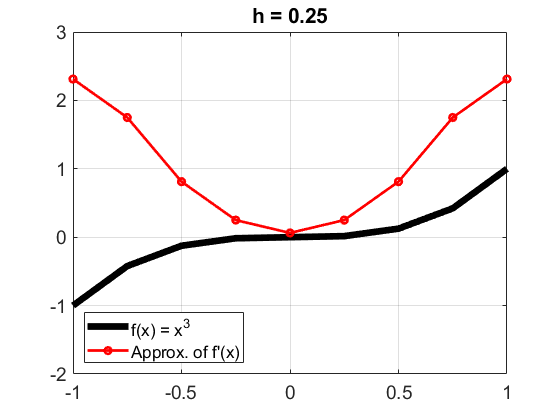
\includegraphics[width=3.5cm]{derivative_h0.25.png} \hspace{0.25cm}
			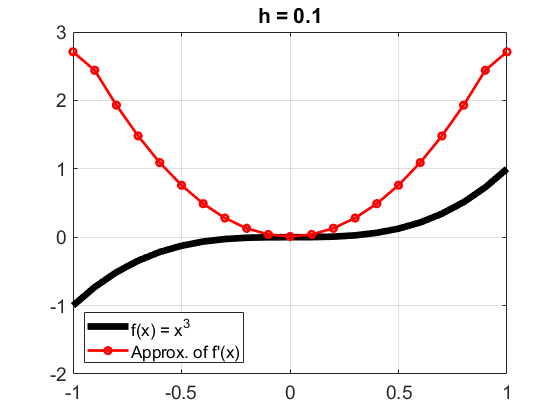
\includegraphics[width=3.5cm]{derivative_h0.1.png} \hspace{0.25cm}
			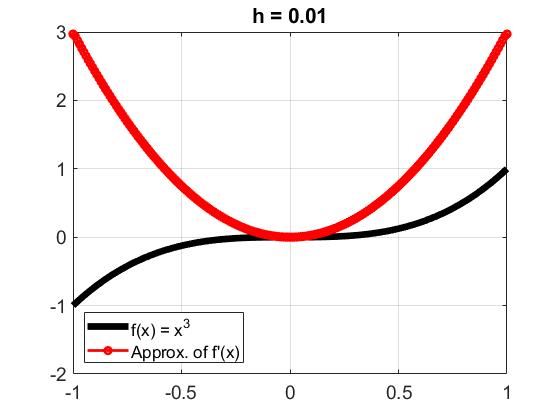
\includegraphics[width=3.5cm]{derivative_h0.01.png} 
		\end{center}
		\item We can see clearly that more points gives us a more accurate estimate 
	\end{itemize}
	
\end{frame}

%%%%%%%%%%%%%%%%%%%%%%%%%%%%%%%%%%%%%%%%%%%%%%%%%%%%%%%%%

\begin{frame}{Speed of an Object}
	\footnotesize
	\begin{columns}
		\begin{column}{0.65\linewidth}
			\begin{itemize}
				\item Suppose we are given some noisy data for the location of an object over time and want to know its speed.
				\item We don't know an underlying function so it seems our only option is to do numerical differentiation!
				\item For example, lets look at some of my GPS data and figure out what I was doing on August 12, 2021
				\begin{itemize}
					\item We have times and a distance traveled, lets get a guess based on my speed
					\item $ v = \frac{9448\text{ m}}{2485.55\text{ s}} \approx 3.8\text{ m/s} = 8.5\text{ mph}$
				\end{itemize}
			\item Based on this information, Google thinks there is a 68.8\% chance I was on a run, and a 17.9\% chance of cycling. Heck there is a 0.01\% chance I was flying!
			\item I was actually rollerblading, so good guess!
			\end{itemize}
		\end{column}
		\begin{column}{0.35\linewidth}
			\begin{center}
				\includegraphics[height = 4cm]{gps_data.png}\\
				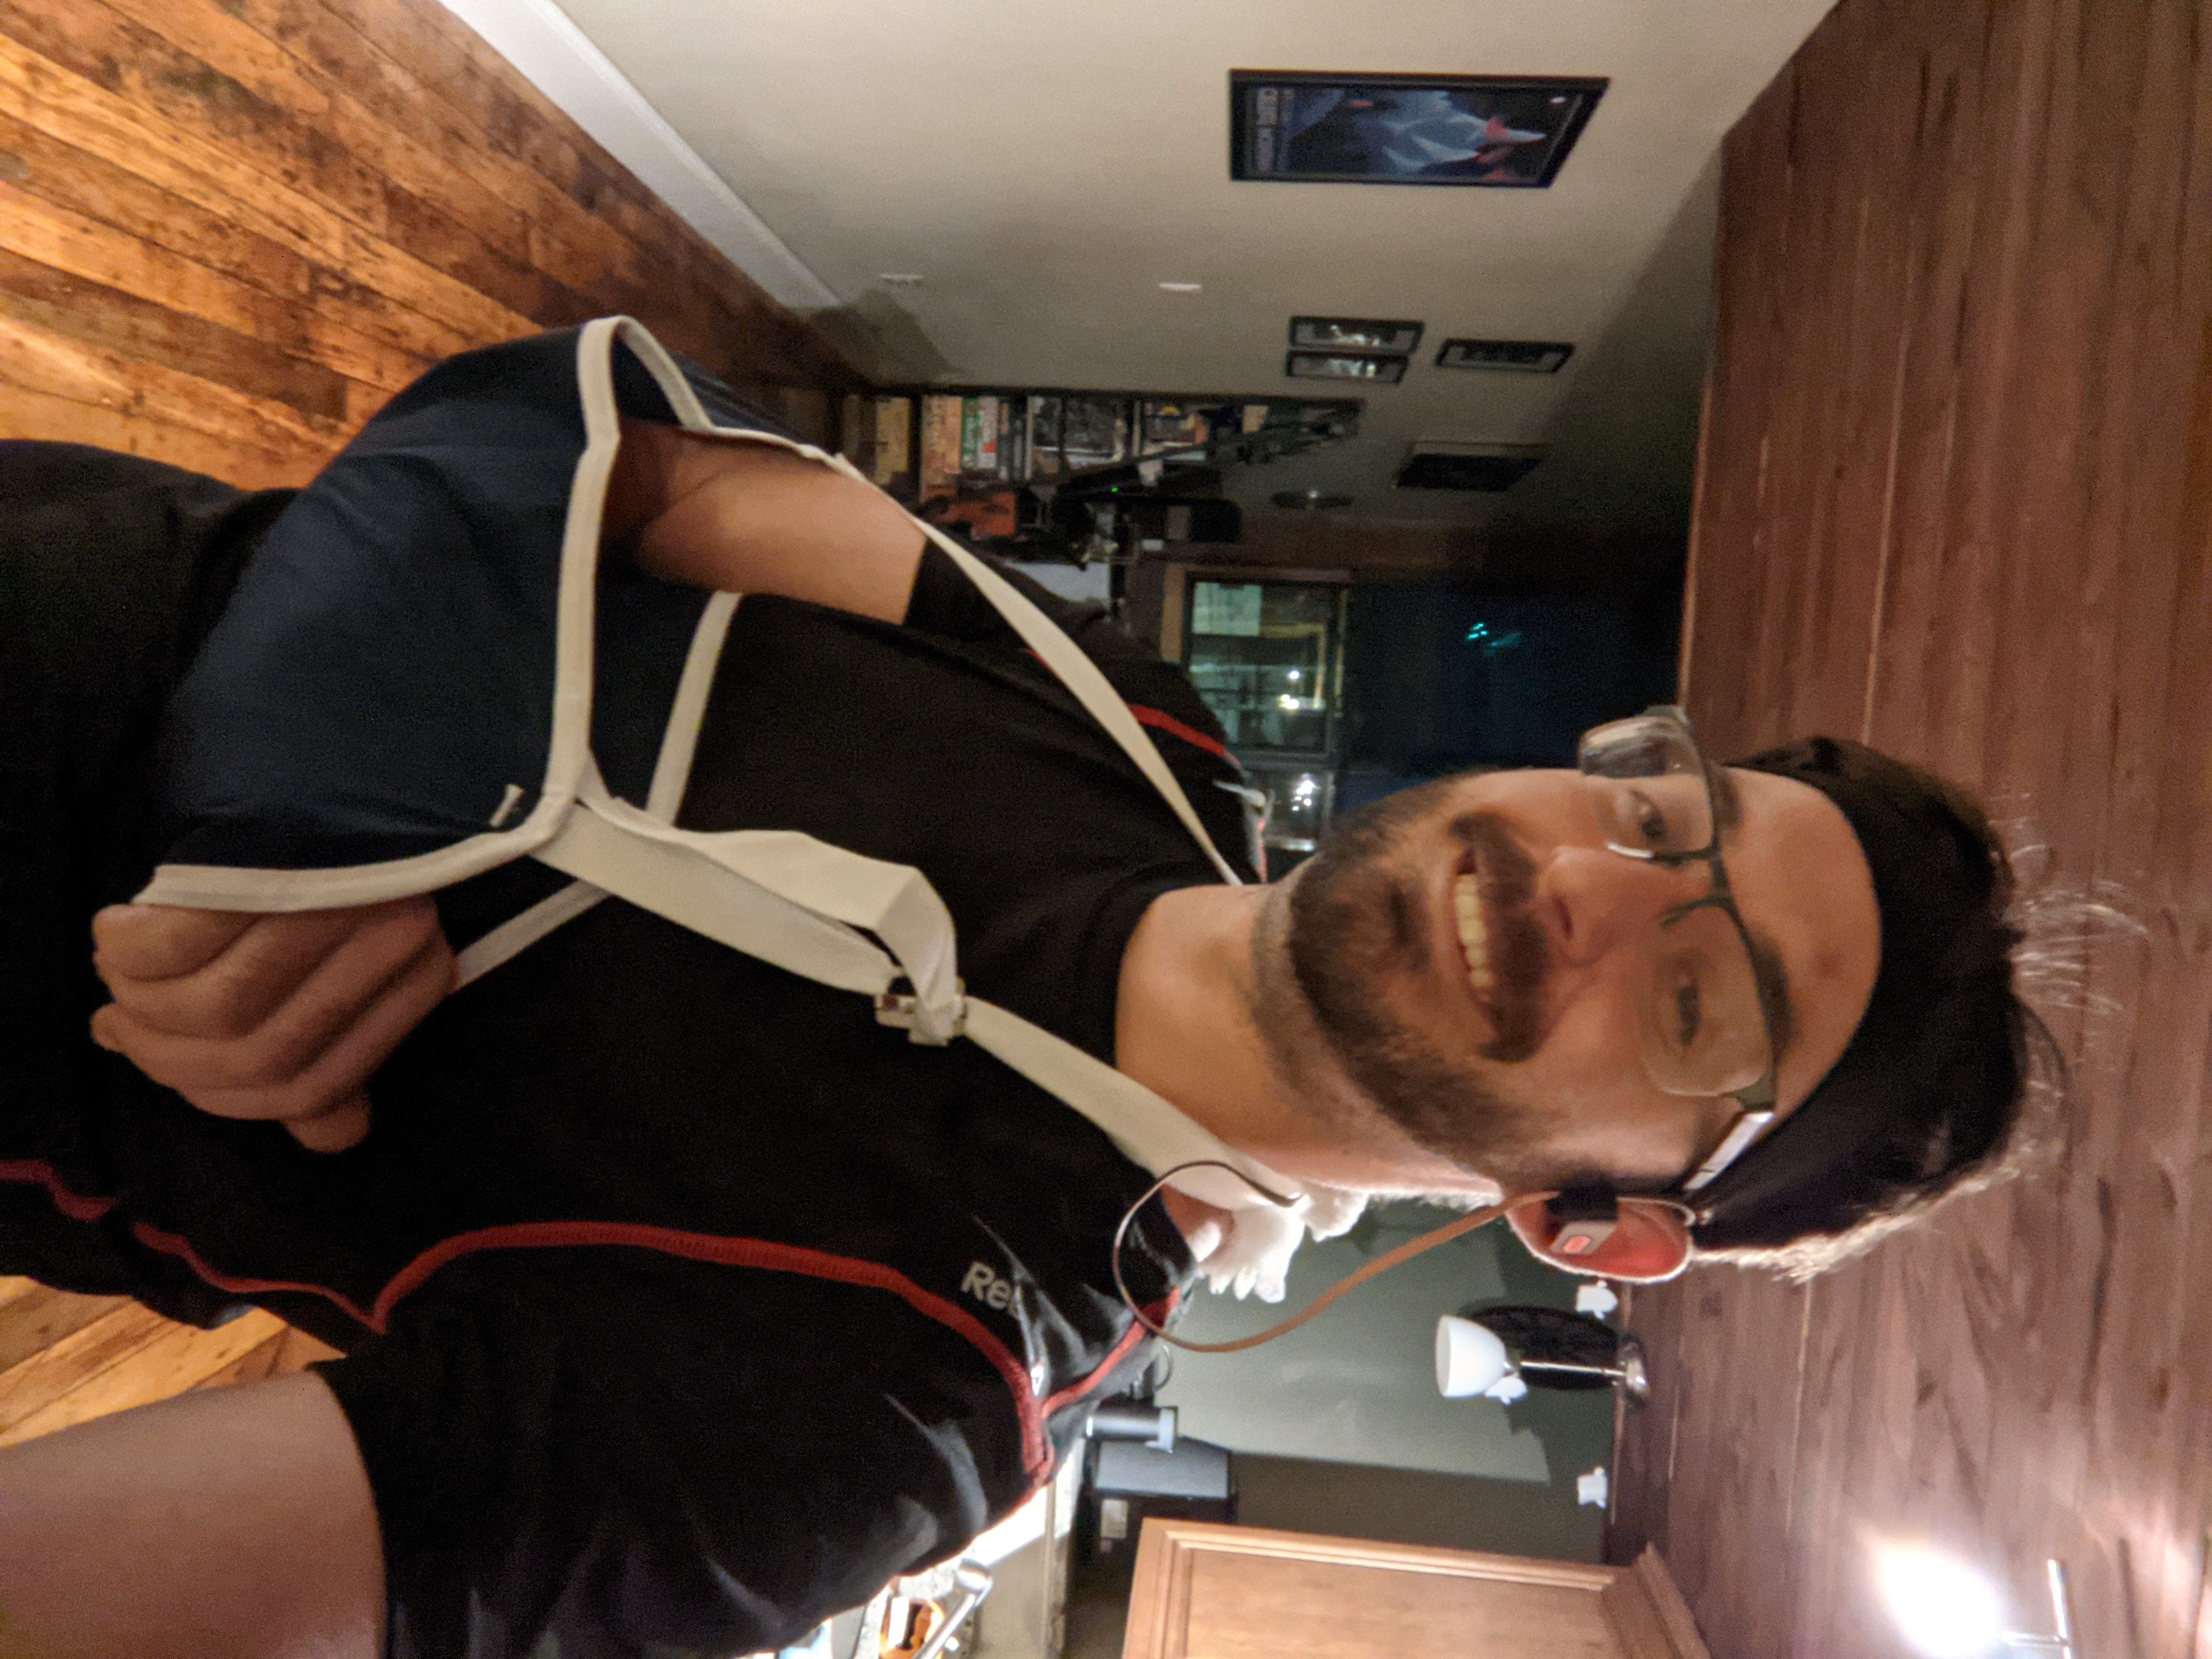
\includegraphics[angle = 90, width = 0.6\linewidth]{Broken_Chris.jpg}\\
			\end{center}
		\end{column}
	\end{columns}
\end{frame}

%%%%%%%%%%%%%%%%%%%%%%%%%%%%%%%%%%%%%%%%%%%%%%%%%%%%%%%%%
\end{document}